\documentclass[journal]{./IEEE/IEEEtran}
\usepackage{cite,graphicx}
\usepackage{url}
\usepackage{listings}

\newcommand{\SPTITLE}{QRSMS: A SMS client with end-to-end encryption via Quick Response (QR) code}
\newcommand{\ADVISEE}{John Mel R. Ramos}
\newcommand{\ADVISER}{Jaderick P. Pabico}

\newcommand{\BSCS}{Bachelor of Science in Computer Science}
\newcommand{\ICS}{Institute of Computer Science}
\newcommand{\UPLB}{University of the Philippines Los Ba\~{n}os}
\newcommand{\REMARK}{\thanks{Presented to the Faculty of the \ICS, \UPLB\
		in partial fulfillment of the requirements
		for the Degree of \BSCS}}
\markboth{CMSC 190 Special Problem, \ICS}{}
\title{\SPTITLE}
\author{\ADVISEE~and~\ADVISER%
	\REMARK
}
\pubid{\copyright~2006~ICS \UPLB}
%%%%%%%%%%%%%%%%%%%%%%%%%%%%%%%%%%%%%%%%%%%%%%%%%%%%%%%%%%%%%%%%%%%%%%%%%%
\begin{document}

% TITLE
\maketitle

% ABSTRACT
%\begin{abstract}
%The quick brown fox jumps over the lazy dog near the riverbank.
%\end{abstract}

% INDEX TERMS
%\begin{keywords}
%SMS, end-to-end encryption
%\end{keywords}

% INTRODUCTION
\section{Introduction}
Despite the emergence of instant messaging (IM) and Over-the-top (OTT)
messaging applications, short message service (SMS) remains as a popular option
for mobile communication. With the first text message sent in 1992 through the
Global System for Mobile communication (GSM) network, the technology has seen
a lot of growth and  development~\cite{LeBodic_2005}. While mostly used for
person-to-person communication \cite{Herring_Stein_Virtanen_2013}, the medium
has seen other applications such as alert notification~\cite{Yoo_Lee_Yoo_Xiao_2021,
	Azid_Sharma_Raghuwaiya_Chand_Prasad_Jacquier_2015},
empowering businesses and online services~\cite{Gargaro_2023, Okazaki_Taylor_2008,
	SecureSMS14}, mobile health (m-health) interventions~\cite{NudgeFlu23, SMSUx22},
mobile government applications~\cite{Onashoga_Ogunjobi_Ibharalu_Lawal_2016, EGov13},
education~\cite{Hill_Hill_Sherman_2007}, Two-Factor Authentication (2FA)
~\cite{DynamicOTP} and more. During the year 2022, Globe Telecom gained
Php 8.8 billion revenue from SMS with 86.7 million mobile customers.
Furthermore, the company has invested Php 1.1 billion to improve spam and
fraudulent SMS detection and prevention~\cite{GlobeIR22}. Unreliable internet
service as well as the lack of Internet infrastructure in some area remains a
challenge in the adoption of online services for communication such as
Facebook Messenger, Viber, Telegram, etc. SMS on the other hand is ubiquitous.
Anyone with a mobile device and a registered subscriber identity module (SIM)
card can send and receive text messages regardless of their platform and
cellular provider~\cite{PhilStar}.

Regardless of its wide range of applications and sustained use, however,
SMS is not ideal for private communication such as sending sensitive and
confidential information as early specifications for SMS does not have security
in mind~\cite{3gpp2}. The European Telecommunications Standards Institute (ETSI)
specified the use of A5 algorithm for encryption over the GSM network together
with the A3 and A8 algorithm for authentication and cipher key generation to
provide security~\cite{Schiller2011} but attacks on the A5/1 and the weaker
A5/2 algorithms has been demonstrated even with minimal resources
~\cite{a512001, a522007,Barkan_Biham_Keller_2003} and even the A5/3 used for
Third Generation (3G) network has been compromised~\cite{a532010}.
Mobile network operators may also opt not to use any encryption during the
transit of message wirelessly~\cite{gsm348}. This means that a
Man-in-the-Middle (MITM) can sit between the Mobile Equipment (ME) and
Base Station Subsystem (BSS) using an International Mobile Subscriber Identity
(IMSI) catcher to actively intercept traffic and even request the victim ME
to use a weaker or no encryption at all~\cite{Cattaneo_DeMaio_Faruolo_Petrillo_2013}.
Additionally, encryption is only performed between the Mobile Equipment (ME)
and the Base Station Subsystem (BSS)~\cite{Schiller2011}. Once the message
reaches the SMS Center (SMSC), messages are stored and kept in plain text for a
while allowing malicious entities to target the SMSC to
view the contents of these messages. This makes an end-to-end encryption a huge
improvement over what is available in the GSM specifications.

To provide a better security system for SMS, independent researchers have
proposed frameworks and protocols that offers end-to-end encryption.
PK-SIM~\cite{PKSIMcard07} provides end-to-end security between the mobile user
and service provider through Public Key Infrastructure (PKI).
SMSSec~\cite{SMSSec08} was developed using the Java Wireless Messaging API (WAP)
and uses a combination of asymmetric and symmetric cryptography to provide
security. EasySMS~\cite{EasySMS14} and SecureSMS~\cite{SecureSMS14} are
completely based on symmetric key cryptography. Similarly, SmartSMS
~\cite{SmartSMS16} uses symmetric key encryption for m-health application.
These protocols however, requires additional resources and infrastructure
on the side of the service provider in order to be implemented.

This paper propose an SMS client that uses
quick-response (QR) codes for key exchange. Initially developed by Toyota's
subsidiary Denso Wave for inventory of vehicle parts manufacturing,
QR code has seen many application in today's era~\cite{Tiwari_2016}.
Able to store up to a maximum of 7,089 characters in one code~\cite{qrcode}
it can be used to encode text, URL, and other data and can be decoded using
a mobile device equipped with a camera and the appropriate software which can
display a text, connect to a wireless network, open a webpage, or open a linked
application~\cite{Shin_Jung_Chang_2012}. The proposed client will encode the
public key and parameters needed to generate a shared secret in a QR code. The
code can be shared to the intended recipient through offline (in person)
or other secure online platform that allows sending of images.

End-to-end security will be achieved through the combined use of symmetric and
asymmetric cryptography as well a key-agreement protocol. Advaned Encryption
Standard (AES) will be used for encrypting the message as it provides the
most security while being performant~\cite{Karale_Pendke_Dahiwale_2015}.
Elliptic Curve Cryptography (ECC) will be used for generating key pairs and
Elliptic Curve Diffie-Hellman (ECDH) for generating a shared secret. The use
of ECC allows for a smaller key length while providing an comparable security
as the Rivest–Shamir–Adleman (RSA) public key cryptosystem
~\cite{Amara_Siad_2011}.

The proposed method will use the android platform to  develop an SMS client
that can generate keypair, exchange public keys through QR code, and establish
an end-to-end encrypted communication.

% REVIEW OF RELATED LITERATURE
\section{Literature Review}
Regardless of the insecurity present in SMS, due to its wide spread
application, it remains to be of use to many users around the world.
To provide better end-to-end security, protocols/frameworks has been proposed.

PK-SIM \cite{PKSIMcard07} card is a framework developed based on Public Key
Infrastructure (PKI) providing end-to-end encryption between the Service
Provider (SP) and the mobile user which contains the PK-SIM card. Their
framework is composed of the mobile client, a Certification Authority and
Registration Authority (CA/RA), a Secure Access gateway (SAG) found in the service provider's infrastructure and the Mobile Operator (MO) that
provides the network for SMS communication. Before the user can send secure
messages, the SAG together, with the CA/RA must first validate the identity
of the mobile client. A primary key shared between the client and the SAG is
generated during the authentication phase. This key is used to establish
a session key which is used to symmetrically encrypt/decrypt the message.
However, in their approach, end-to-end security is only available between
the mobile client and the SAG on the Service Provider's side. Additionally,
it is stated that the generation of primary key in the authentication phase
takes up to a day or longer. Every time this key expires, the protocol must
be performed again from the beginning. Similarly, the SMSSec~\cite{SMSSec08}
protocol is designed such that it uses a combination of asymmetric
cryptography for authenticating the user and uses symmetric cryptography
for the actual exchange of messages. It also falls short such that
end-to-end encryption is between the mobile device and the authentication
source. Unlike PK-SIM however, SMSSec is a software solution built with
the Java Wireless Messaging API (WAP).

In contrast, the EasySMS \cite{EasySMS14} protocol is designed to provide
end-to-end encryption using only symmetric algorithm. In their approach,
an Authentication Server (AS) is responsible for the storage of all secret key
shared between the AS and the respective Mobile Station (MS) or the user.
It is also assumed that there is a shared secret key between the AS and a
CA/RA which contains information about every mobile subscriber. Before a SIM
card could be used, a subscriber must first register within the CA/RA. With
these requirements met, the AS, with the help of CA/RA can now authenticate
any MS that wants to send an SMS securely. However, this approach falls under
the same disadvantage as the previous protocols. When user A wants to send a message to user B, the AS validates the identity of both users and generate
different key for each respective user. This means that the message from
user A is encrypted with the key shared between the AS and user A, decrypted
in the AS then re-encrypt the message for user B using the key shared between
the AS and user B. This approach is also used for the development of
SecueSMS~\cite{SecureSMS14} but is proposed to be specific for value added
services (VAS) and commercial applications. SmartSMS~\cite{SmartSMS16} follows
a similar concept but instead of the AS being connected to a CA/RA, a
trusted third party hosted in a public cloud is responsible for the
functions of CA/RA.

In these protocol, apart from being not truly end-to-end encrypted (encryption
only occurs between the mobile station and the service provider), they also
require a third party for authenticating the user. This means that in order to
achieve secure communication, changes within the service provider's and the
network itself must be consider. This paper will introduce a
different approach that does not require additional infrastructure by
having the ciphertext sent through the SMS network while encryption and
decryption is performed by the communicating devices.

\section{Objectives}
To create a secure platform for the exchange of encrypted SMS, the main
objective of this research is to develop an SMS client application that
can encrypt and decrypt messages and utilize QR codes as means of
exchanging keys for generating a shared secret. To be specific, this research
aims to do the following:
\begin{itemize}
	\item[1.] Design and implement a key-agreement protocol using QR code
		as means for key exchange.
	\item[2.] Design and implement an SMS client for mobile android device  with
		end-to-end encryption.
	\item[3.] Conduct a usability study of the SMS client application.
\end{itemize}

\begin{figure*}
	\centering
	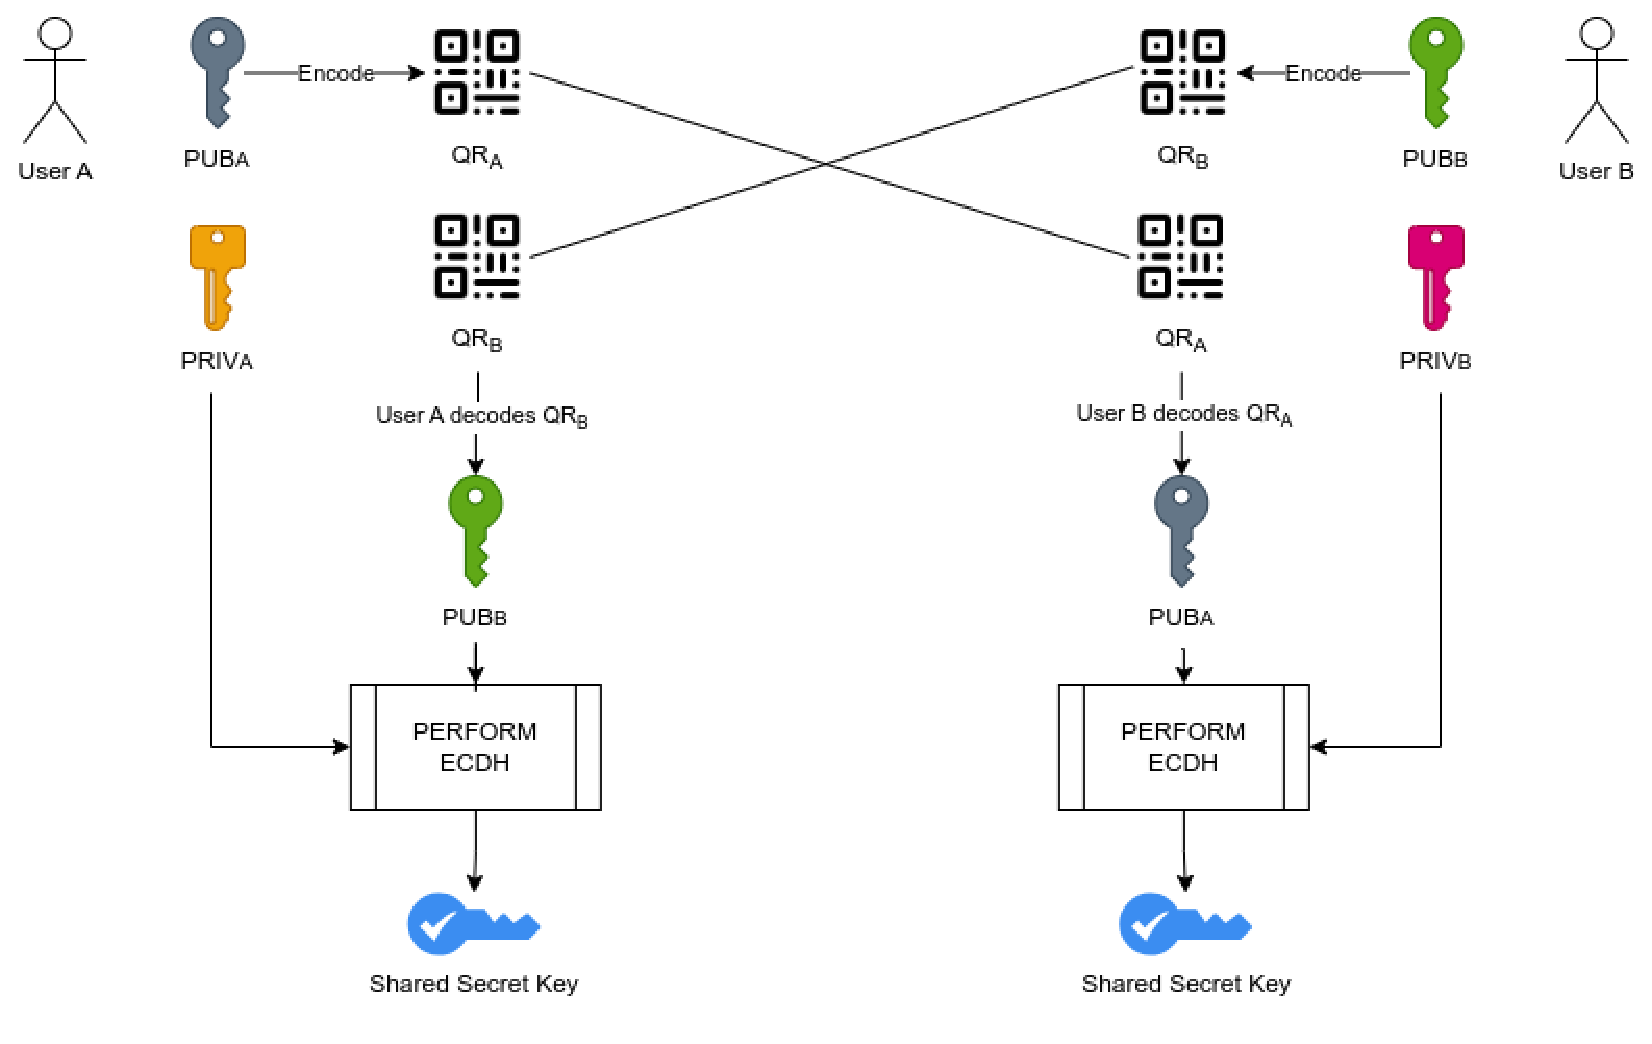
\includegraphics[width=6in]{images/key_agreement.eps}
	\caption{Overview of key generation and key agreement in QRSMS}
	\label{key_genagree}
\end{figure*}

\begin{figure*}
	\centering
	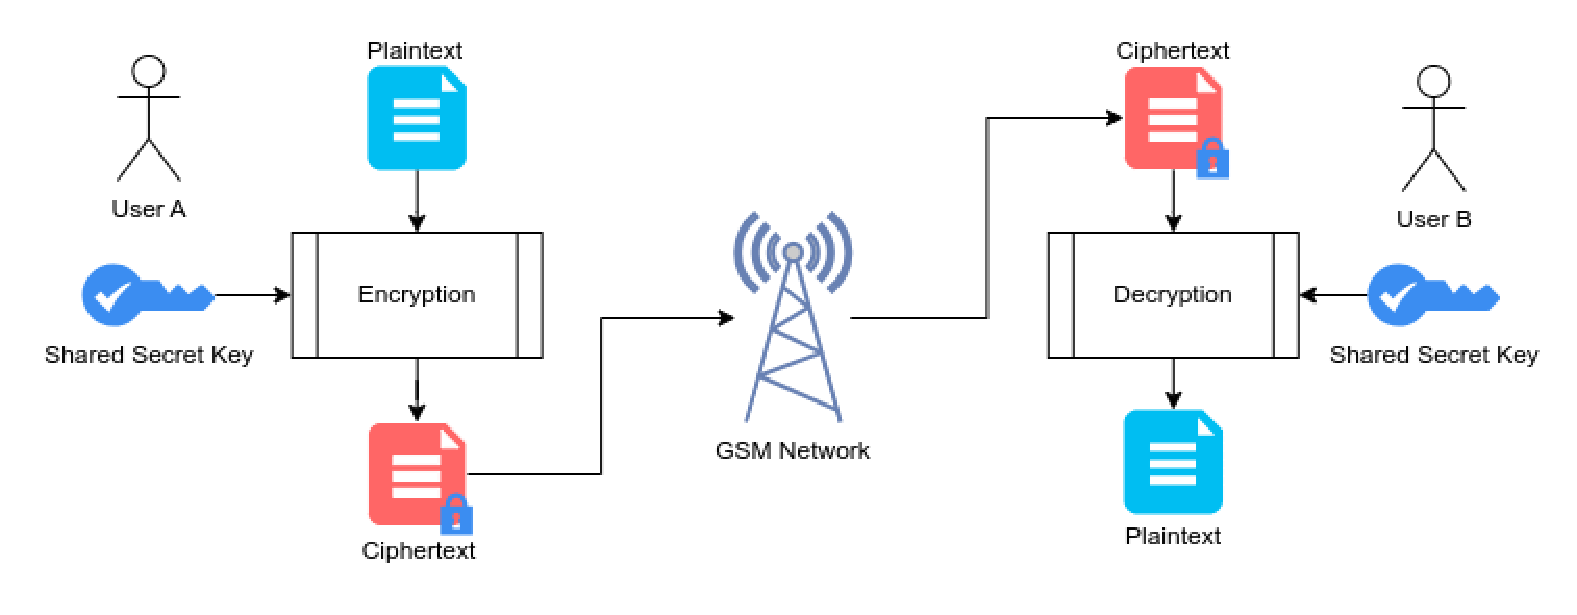
\includegraphics[width=6in]{images/encrypted_messaging.eps}
	\caption{Overview of sending and decryption of messages in
		QRSMS}
	\label{encrypted}
\end{figure*}

\section{Materials and Methods}
%% [1.] Design and implement a key-agreement protocol using QR code
\subsection{Key-Agreement Protocol}
To achieve end-to-end security, participants in the exchange should be able to
generate a shared key known only to them. This process can be further divided
into two steps. Keypair generation and shared secret key generation. This two
step process is shown in Figure \ref{key_genagree}.
The \lstinline{javax.crypto} library contains the KeyAgreement class needed to
establish a shared secret while the \lstinline{java.security} library
will enable us to use the KeyGenerator class which allows the generation of
public and private key pair using EC. Since there are no built-in libraries
for encoding and decoding of QR code, ZXing~\cite{zxing} and Google's ML
kit barcode scanning~\cite{mlkit} will be bundled with the application to
provide the missing functionalities.

\subsubsection{Keypair Generation}
To be able to generate a shared secret with another user, each party involved
must first generated their public and private key pair. For each contact the
user wants to exchange keys with, a unique key pair will be generated
using Elliptic Curve (EC) algorithm.
The generated public key will be encoded to a QR code while the complementing
private key will be kept securely in the system and will be used to finalize
the key exchange.

\subsubsection{Shared Secret key Generation}
Once each party have their generated QR code, they will give their QR code to
the each other and scan the code to retrieve the key. Using ECDH,
their private key for that particular user will be fed along with the scanned
public key to generate a shared secret. This process is illustrated in
fig.~\ref{key_genagree}.
The shared secret will be stored inside Android's built in KeyStore to protect
the keys from unauthorized use~\cite{android_keystore}.

It should be noted that in order to keep the integrity of the system,
an assumption is made that the user will not feed a QR code
whose origin is unknown. To ensure that the code being decoded is from the
intended contact, the QR code should only come from the other party involved
in the secure communication through other means such as offline
(in-person exchange) or secure online application. This eliminates the need
for authentication methods as the users themselves are the one responsible
for ensuring that the participant in the exchange is the intended receipient.
%% [2.] Design and implement an SMS client for mobile android device  with
%% 	end-to-end encryption.
\subsection{Encrypted Messaging}
To enable end-to-end encryption, both the sending and receiving party must
have the application installed and have exchanged their QR code generated by
the application through other means suggested below. In case only one party
has the software installed, if they decide to send an encrypted message to
a user without the application, or the receipient have not yet established the
shared secret, the latter might receive the message in
ciphertext, unable to read said text. If the opposite were to occur,
the application should be able to determine if the received text was encrypted
or not.

When each of the user involved in the key-agreement now having generated a
shared secret with their intended contact, the exchange of encrypted SMS
can now begin. AES encryption algorithm can be used generate the ciphertext
with the shared secret as the key for symmetric cryptography shown in
fig.~\ref{encrypted}. The android platform comes with the
\lstinline{android.telephony} package contains the classes needed for sending
and receiving SMS messages while the \lstinline{javax.crypto} contains
classes that allows the use ofcryptographic libraries that will help achieve
the goals of the application~\cite{android_pkg}.

Equipped with features and support for developing android applications,
Android Studio will be used as the integrated development environment (IDE)
to facilitate the development of the SMS client.
The Kotlin programming language will also be used for the application as it
fully supported for android development and it eliminates the verbosity
of Java while allowing the use of Java libraries
~\cite{Moskala_Wojda_2017}.

%% [3.] Conduct a usability study of the SMS client application.
\subsection{User Testing}
Throughout the duration of the development process, the features and interface
of the system will be thoroughly tested to ensure that the program can perform
its intended functions. However, upon the completion of a minimum viable
product, usability test will be conducted to further inspect the working
condition off the application as well as analyze users' thoughts with regards
to the system. Users will be asked to perform various tasks that involves the
following capabilities of the application:

\begin{figure}
	\centering
	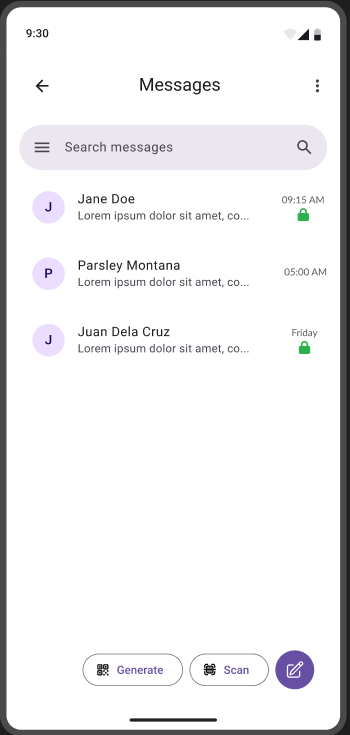
\includegraphics[height=3.5in]{./images/QRSMS_inbox.png}
	\caption{QRSMS Inbox UI Prototype}
	\label{QRSMSUI}
\end{figure}

\begin{itemize}
	\item[1.] Generation of QR code containing the public key to be used for
		a contact
	\item[2.] Scanning and decoding of QR code received from a contact
	\item[3.] Sending of unencrypted and encrypted messages
	\item[4.] Reading of unencrypted and encrypted messages
	\item[5.] Management of stored keys
\end{itemize}

Along with the given tasks are questionnaire that aims to understand users'
perspective throughout their usage of the application. Single Ease Question
(SEQ) will be asked after completing each task. With measures of central
tendency, a general sentiment can be derived on how well the users performed
in each of the tasks. This can provide an insight on the ease-of-use of the
system. This is followed by a System Usability Scale (SUS) Questionnare
to assess the system's perceived usability.

\section{Expected Outcome}
\subsection{Key-agreement with QR Code}
Behind the SMS client's ability to conceal the contents of each messages, the
key-agreement protocol's function is vital to generate the secret key that
will be used to encrypt each messages. Figure \ref{generate_view} shows the
sequence of views that the user can see when they tap the generate QR in the
inbox user interface (UI). On the other hand, when scanning a QR code,
the sequence of views during this action is shown in figure \ref{scan_view}.
When users A and B wants to send each other encrypted messages, User A must
first generate a QR code intended for user B and provide them the code and
vice-versa. Through this exchange, one of the following cases may occur.

\begin{figure*}
	\centering
	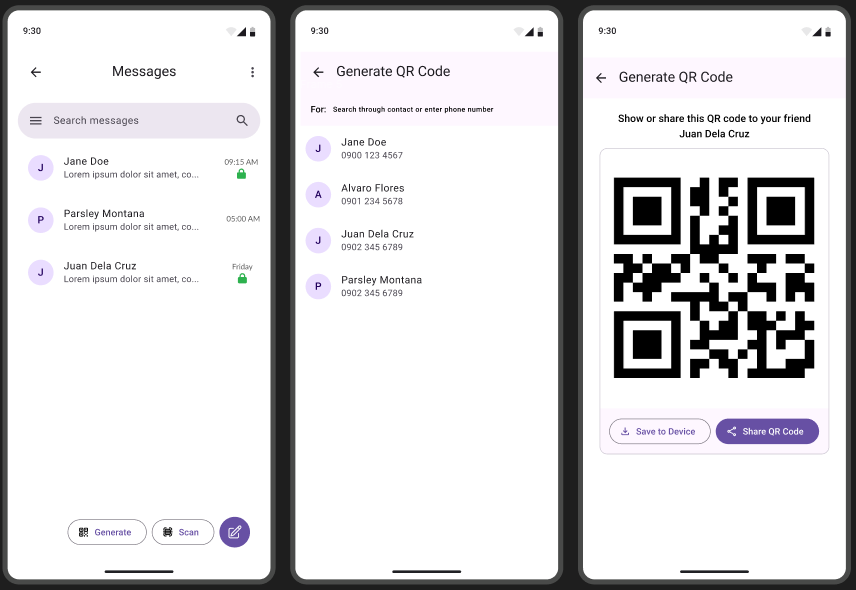
\includegraphics[height=3.5in]{./images/Generate_QR_prototype.png}
	\caption{QR Code generation view prototype}
	\label{generate_view}
\end{figure*}

\begin{figure*}
	\centering
	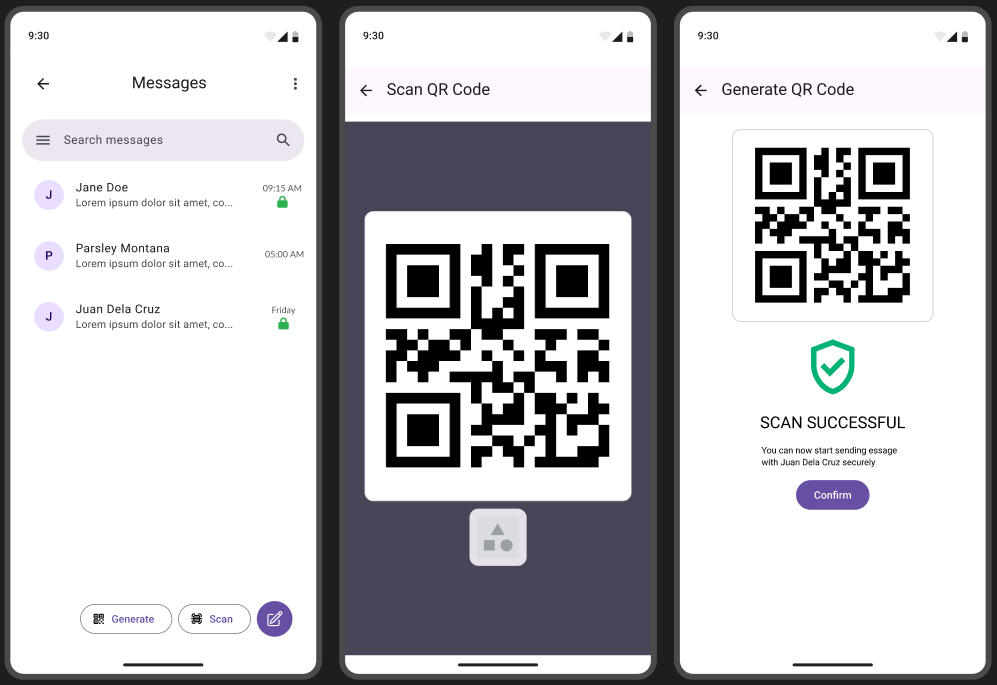
\includegraphics[height=3.5in]{./images/Scan_QR_prototype.png}
	\caption{QR Code scan view prototype}
	\label{scan_view}
\end{figure*}

\subsubsection{Case 1: User A and B receives the correct code}
In this case, when user A generated a QR code they correctly supplied user B's
phone number and gave them the correct QR code. User B does the same and upon
scanning each others given code, the key-agreement protocol is done succesfully
and came up with the same secret key for both user. Encrypted SMS can now
occur.

\subsubsection{Case 2: User A or User B or Both receives the wrong code}
In this case, during generation or sending of QR code, either user A or
user B selected the incorrect phone number or supplied the incorrect QR code.
If this happened, the application should throw a user friendly error message
to allow them to troubleshoot the issue and take appropriate action.

\subsection{SMS Client}
Built for the android operating system, QRSMS is an SMS client that enables
users to exchange end-to-end encrypted messages while allowing them to
send regular SMS if they choose to. To ensure seamless operation by the
user, the system should be designed with a simple and user-friendly interface
such that users of any background can make operate the application without
much difficulty. Figure~\ref{QRSMSUI} shows a prototype of the UI upon entering
the application in which most of the significant functions
of the system should be present and apparent. While users should be able to
choose to send a regular or secure SMS, the system should be able to recognize
if the message is encrypted or not and transform it if necessary to make it
readable by the user.

In general, for the SMS client perform its intended function, the following
requirements must be considered. The application should be able to:
\begin{itemize}
	\item[1.] Encrypt and send SMS message.
	\item[2.] Decrypt and read SMS message.
	\item[3.] Generate a private and public key pair then encode it into a
		QR Code.
	\item[4.] Decode the QR code to generate the shared secret.
	\item[5.] Allow users to manage saved keys.
\end{itemize}

\subsection{Understanding System Usability and Ease of Use}
In general, user testing allows for understanding how a system performs in
real world applications. Having users test and evaluate the system enables
the researchers to recognize the potential of the proposed approach.
With the way the key-agreement protocol is designed, users might initially
find this method different from what they are used to. Users has to initiate
the exchange themselves with the QR code to simplify the act of inputting of
keys. But an intuitive and well designed interface should be able to guide
the users to take their intended actions. Because of the popularity of QR code,
users generally recognizes it and knows how to use it. However, knowing what
aspect of the system users found the most useful and
easy to operate can help identify further improvements to be made.

% APPENDICES
%\appendices

%\section{Proof of the First Zonklar Equation}
%Appendix one text goes here...
%
%\section{}
%Appendix two (without title) text goes here...

% ACKNOWLEDGMENT
%\section*{Acknowledgment}
%Many thanks to...

% BIBLIOGRAPHY
\bibliographystyle{./IEEE/IEEEtran}
\bibliography{./ramos-cs190-ieee}
% \nocite{*}

% BIOGRAPHY
%\begin{biography}[{\includegraphics{./yourPicture.eps}}]{Student M. Name}
%Biography text here...
%\end{biography}

\end{document}
